\section{Stability and the Goldilocks Surface} \label{sec:stability}

The FSA-v3 model, being a 4D non-linear stochastic system, requires careful stability analysis to ensure that the control and inference tasks are well-posed. This analysis follows the roadmap outlined in the \textit{Project Development Plan - FSA-v3 Bimodal Training Extension} and the \textit{Structural Identifiability and FIM Analysis} documents provided in the workspace.

\subsection{The Deterministic Skeleton and Bimodal Bifurcation}

To understand the long-term behavior of the SDE, we analyze its **deterministic skeleton**. This is a standard pedagogical technique where we set the diffusion terms $\sigma_i = 0$ and assume constant training stimuli $\Phi = (\Phi_B, \Phi_S)^T$. This allows us to locate the system's equilibria—the points where the body would eventually settle under a consistent training load.

The steady-state values $(B^*, S^*, F^*)$ are found by setting the drift equations to zero. At the operating point $A = A_{\mathrm{typ}}$, the equations simplify to:
\begin{equation}
    B^* = \text{clip}(\kappa_B \Phi_B \tau_B, 0, 1), \quad S^* = \text{clip}(\kappa_S \Phi_S \tau_S, 0, 1), \quad F^* = (\kappa_{FB} \Phi_B + \kappa_{FS} \Phi_S) \tau_F
\end{equation}

The resulting "Goldilocks" structure is visualized as a 2D surface in stimulus space using the tool \path{tools/generate_stability_data.py}. This script evaluates the Stuart-Landau growth rate $\mu(B^*, S^*, F^*)$ across a grid of $(\Phi_B, \Phi_S)$ and computes the equilibrium amplitude $A^* = \sqrt{\max(\mu, 0)/\eta}$.

\begin{figure}[h]
    \centering
    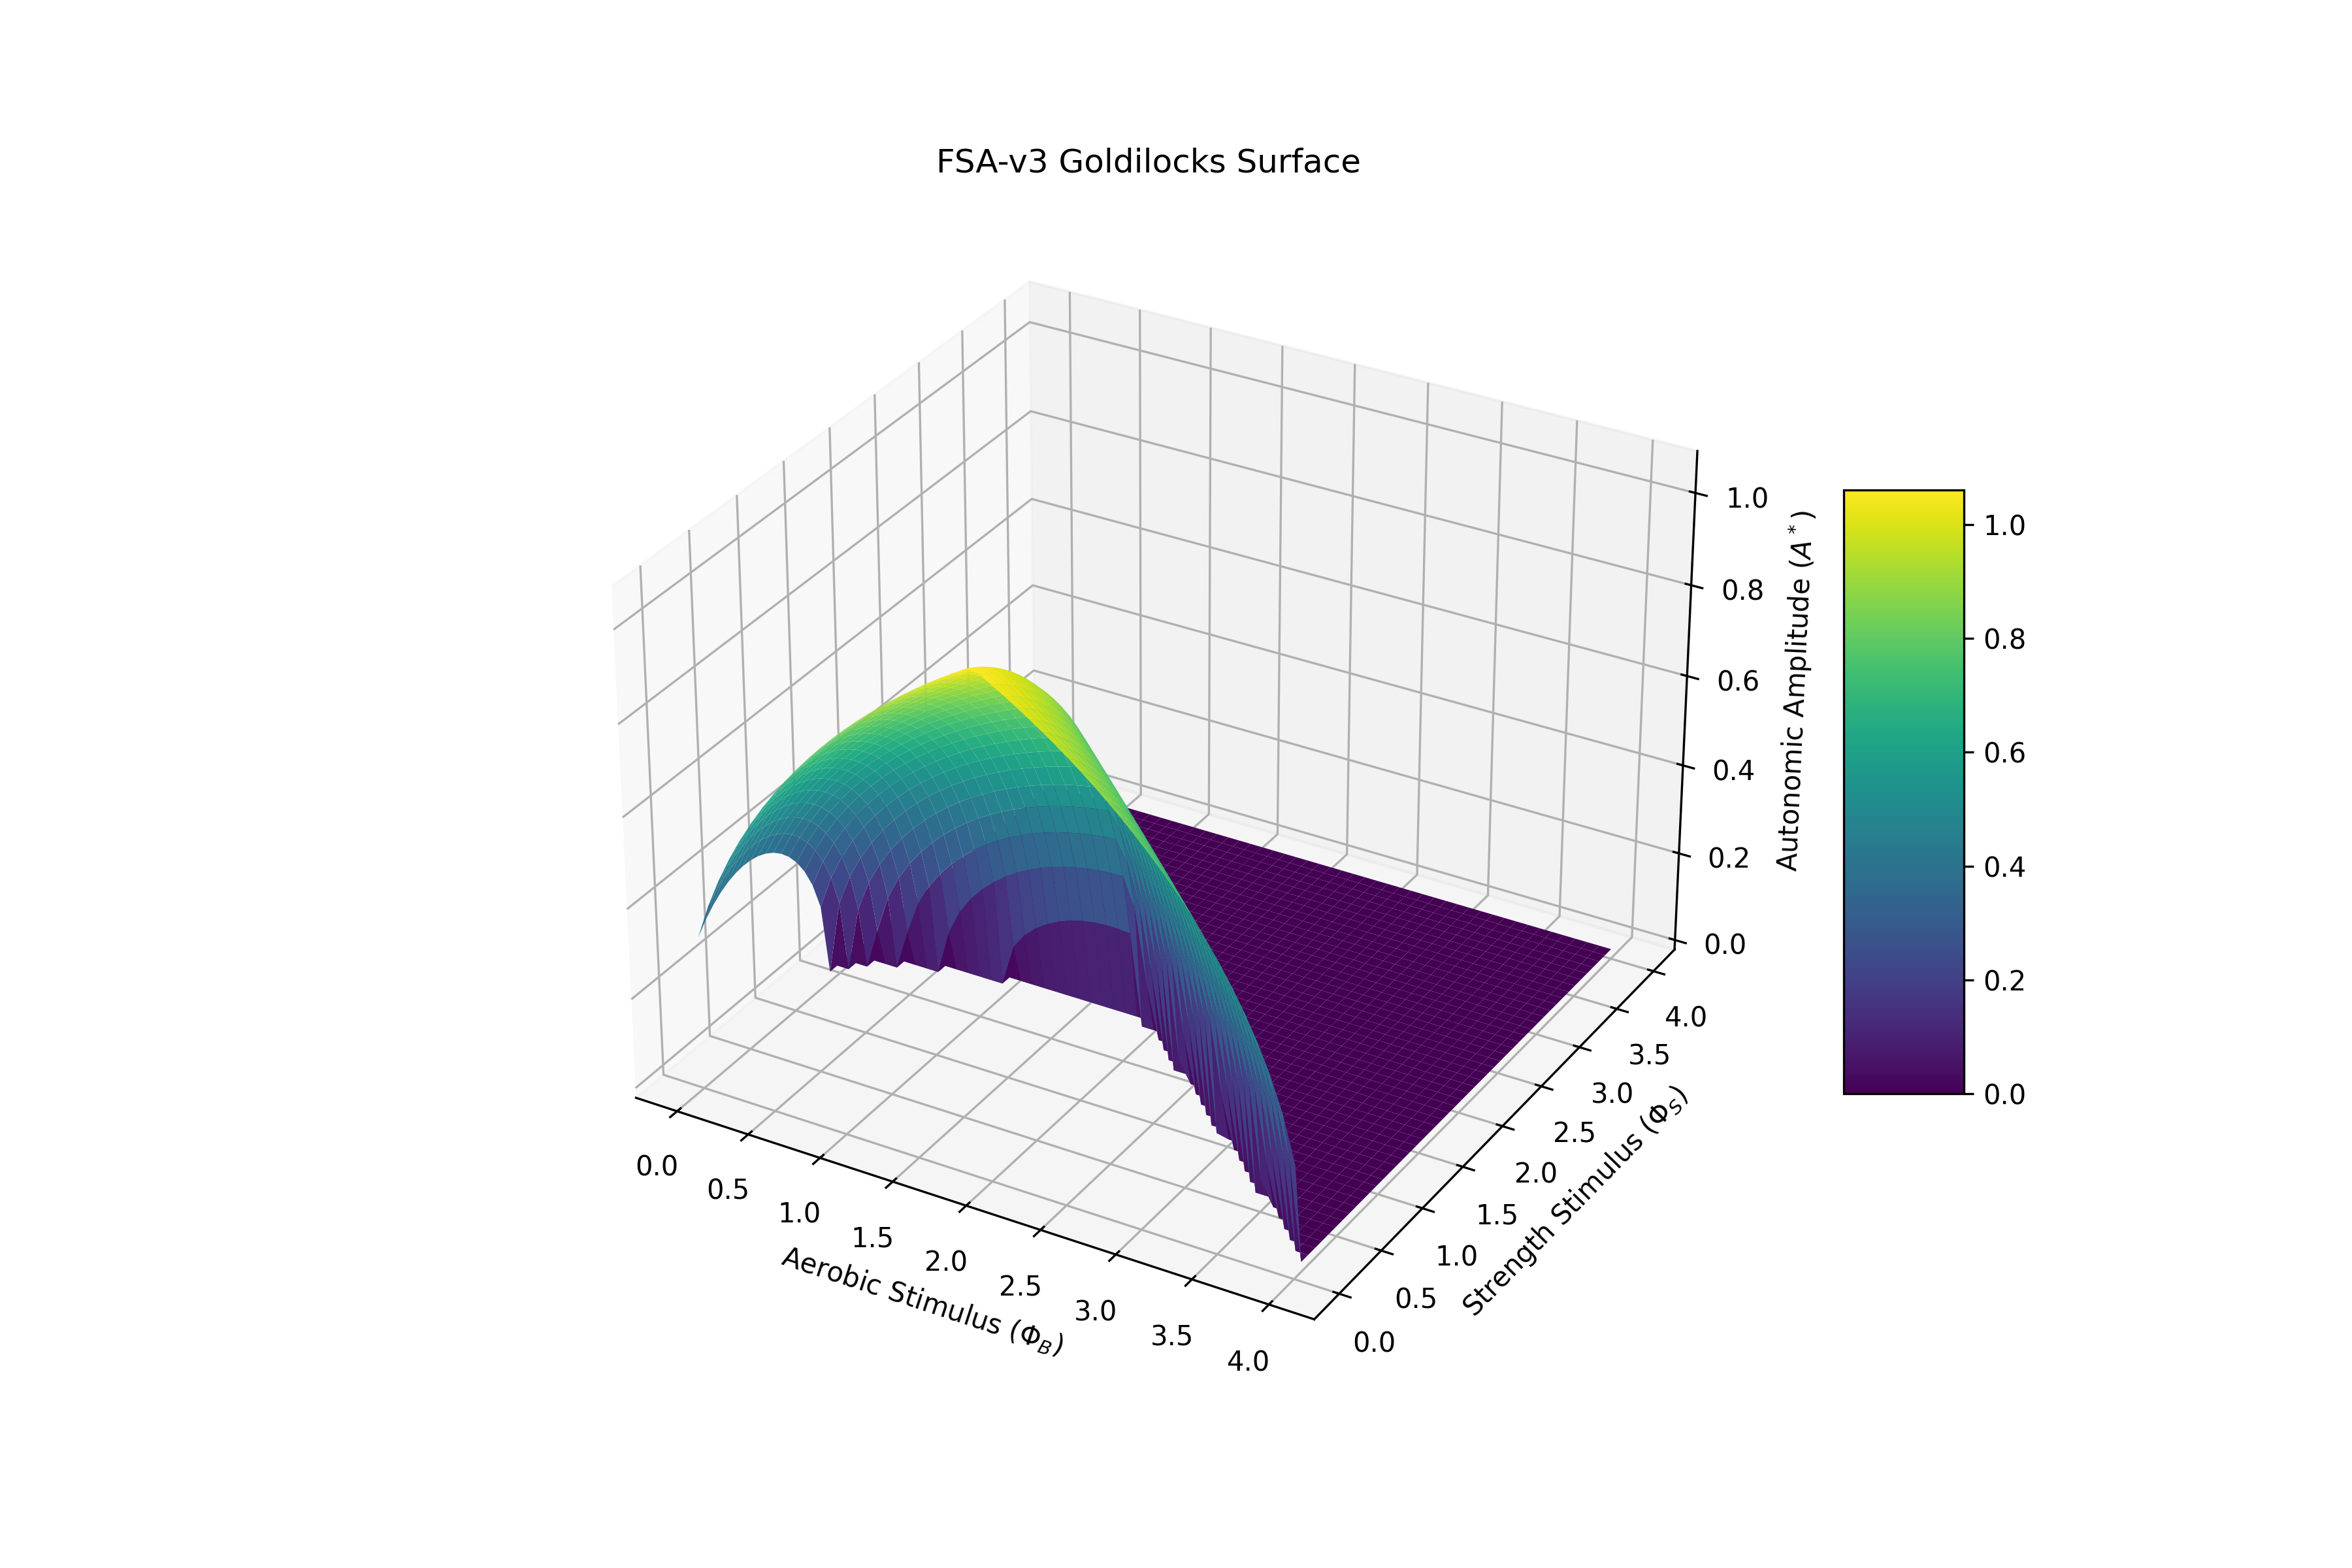
\includegraphics[width=0.8\textwidth]{figures/goldilocks_surface_v3.png}
    \caption{The FSA-v3 Goldilocks Surface. This plot, generated via generate\_stability\_data.py, reveals the bi-modal stability region. As confirmed in the FIM Analysis document, the non-linear coupling $\mu_S S A$ is what allows the system to distinguish between modalities even with sparse observations.}
    \label{fig:goldilocks_surface}
\end{figure}

\subsection{Steady-State Operating Points and the Control Dilemma}

Table \ref{tab:stability_values} provides selected values from the Goldilocks surface. A critical observation arises from these steady states: because strength training ($\Phi_S$) incurs a higher fatigue penalty ($\kappa_{FS} = 0.05$) than aerobic training ($\kappa_{FB} = 0.03$), a controller that only maximizes $\int A \, dt$ will naturally favor aerobic-heavy schedules. 

In this general health regime, strength adaptation is viewed by the optimizer as an "expensive" way to stabilize the autonomic oscillator. This highlights a fundamental distinction between optimizing for \textbf{general wellness} (maximizing $A$) and \textbf{athletic performance} (concurrently maximizing $B$ and $S$).

\begin{table}[h]
\centering
\small
\begin{tabular}{@{}ccccccc@{}}
\toprule
$\Phi_B$ & $\Phi_S$ & $B^*$ & $S^*$ & $F^*$ & $\mu$ & $A^*$ \\
\midrule
0.0 & 0.0 & 0.000 & 0.000 & 0.000 & +0.020 & 0.316 \\
1.0 & 0.0 & 0.513 & 0.000 & 0.187 & +0.141 & 0.841 \\
2.0 & 0.0 & 1.000 & 0.000 & 0.390 & +0.220 & 1.050 \\
0.0 & 1.0 & 0.000 & 0.480 & 0.312 & +0.022 & 0.331 \\
1.0 & 1.0 & 0.513 & 0.480 & 0.499 & +0.097 & 0.695 \\
2.0 & 1.0 & 1.000 & 0.480 & 0.701 & +0.125 & 0.791 \\
0.0 & 2.0 & 0.000 & 0.999 & 0.649 & -0.064 & 0.000 \\
\bottomrule
\end{tabular}
\caption{Steady-state values. Notice how $A^*$ drops significantly when adding $\Phi_S$ to a fixed $\Phi_B$, due to the steeper fatigue gain.}
\label{tab:stability_values}
\end{table}

\subsection{Concurrent Training Cost Functional}

To align the model with the goals of concurrent training—maximizing both cardiovascular and neuromuscular capacities—we recommend a composite cost functional. By rewarding the areas under $B$ and $S$ alongside $A$, we provide the MPC with explicit "performance targets."

The proposed functional is:
\begin{equation}
    J(\theta) = \mathbb{E} \left[ \int_{0}^{T} -(A(t) + \gamma_B B(t) + \gamma_S S(t)) \, dt + \lambda_F \int_{0}^{T} \max(F(t)-F_{\text{max}}, 0)^2 \, dt \right]
\end{equation}

This formulation ensures that the controller pushes the athlete toward their genetic limits ($B \to 1, S \to 1$) while $A$ acts as a safety-informed "health budget" that forces the optimizer to find the most efficient periodization to avoid collapse.

\subsection{Static Optimization: The Concurrent Training Optimum}

To provide pedagogical intuition for the behavior of the new cost functional, we perform a \textbf{static optimization scan}. We treat the stimuli $\Phi_B$ and $\Phi_S$ as constant over an infinite horizon and seek the point on the stimulus plane that maximizes the steady-state concurrent reward $R(\Phi_B, \Phi_S) = A^* + B^* + S^*$.

This analysis, implemented in \path{tools/static_optimization_scan.py}, reduces the dynamic optimal control problem to a search over a 2D landscape. Figure \ref{fig:reward_surface} visualizes this landscape, showing a clear global maximum.

\begin{figure}[h]
    \centering
    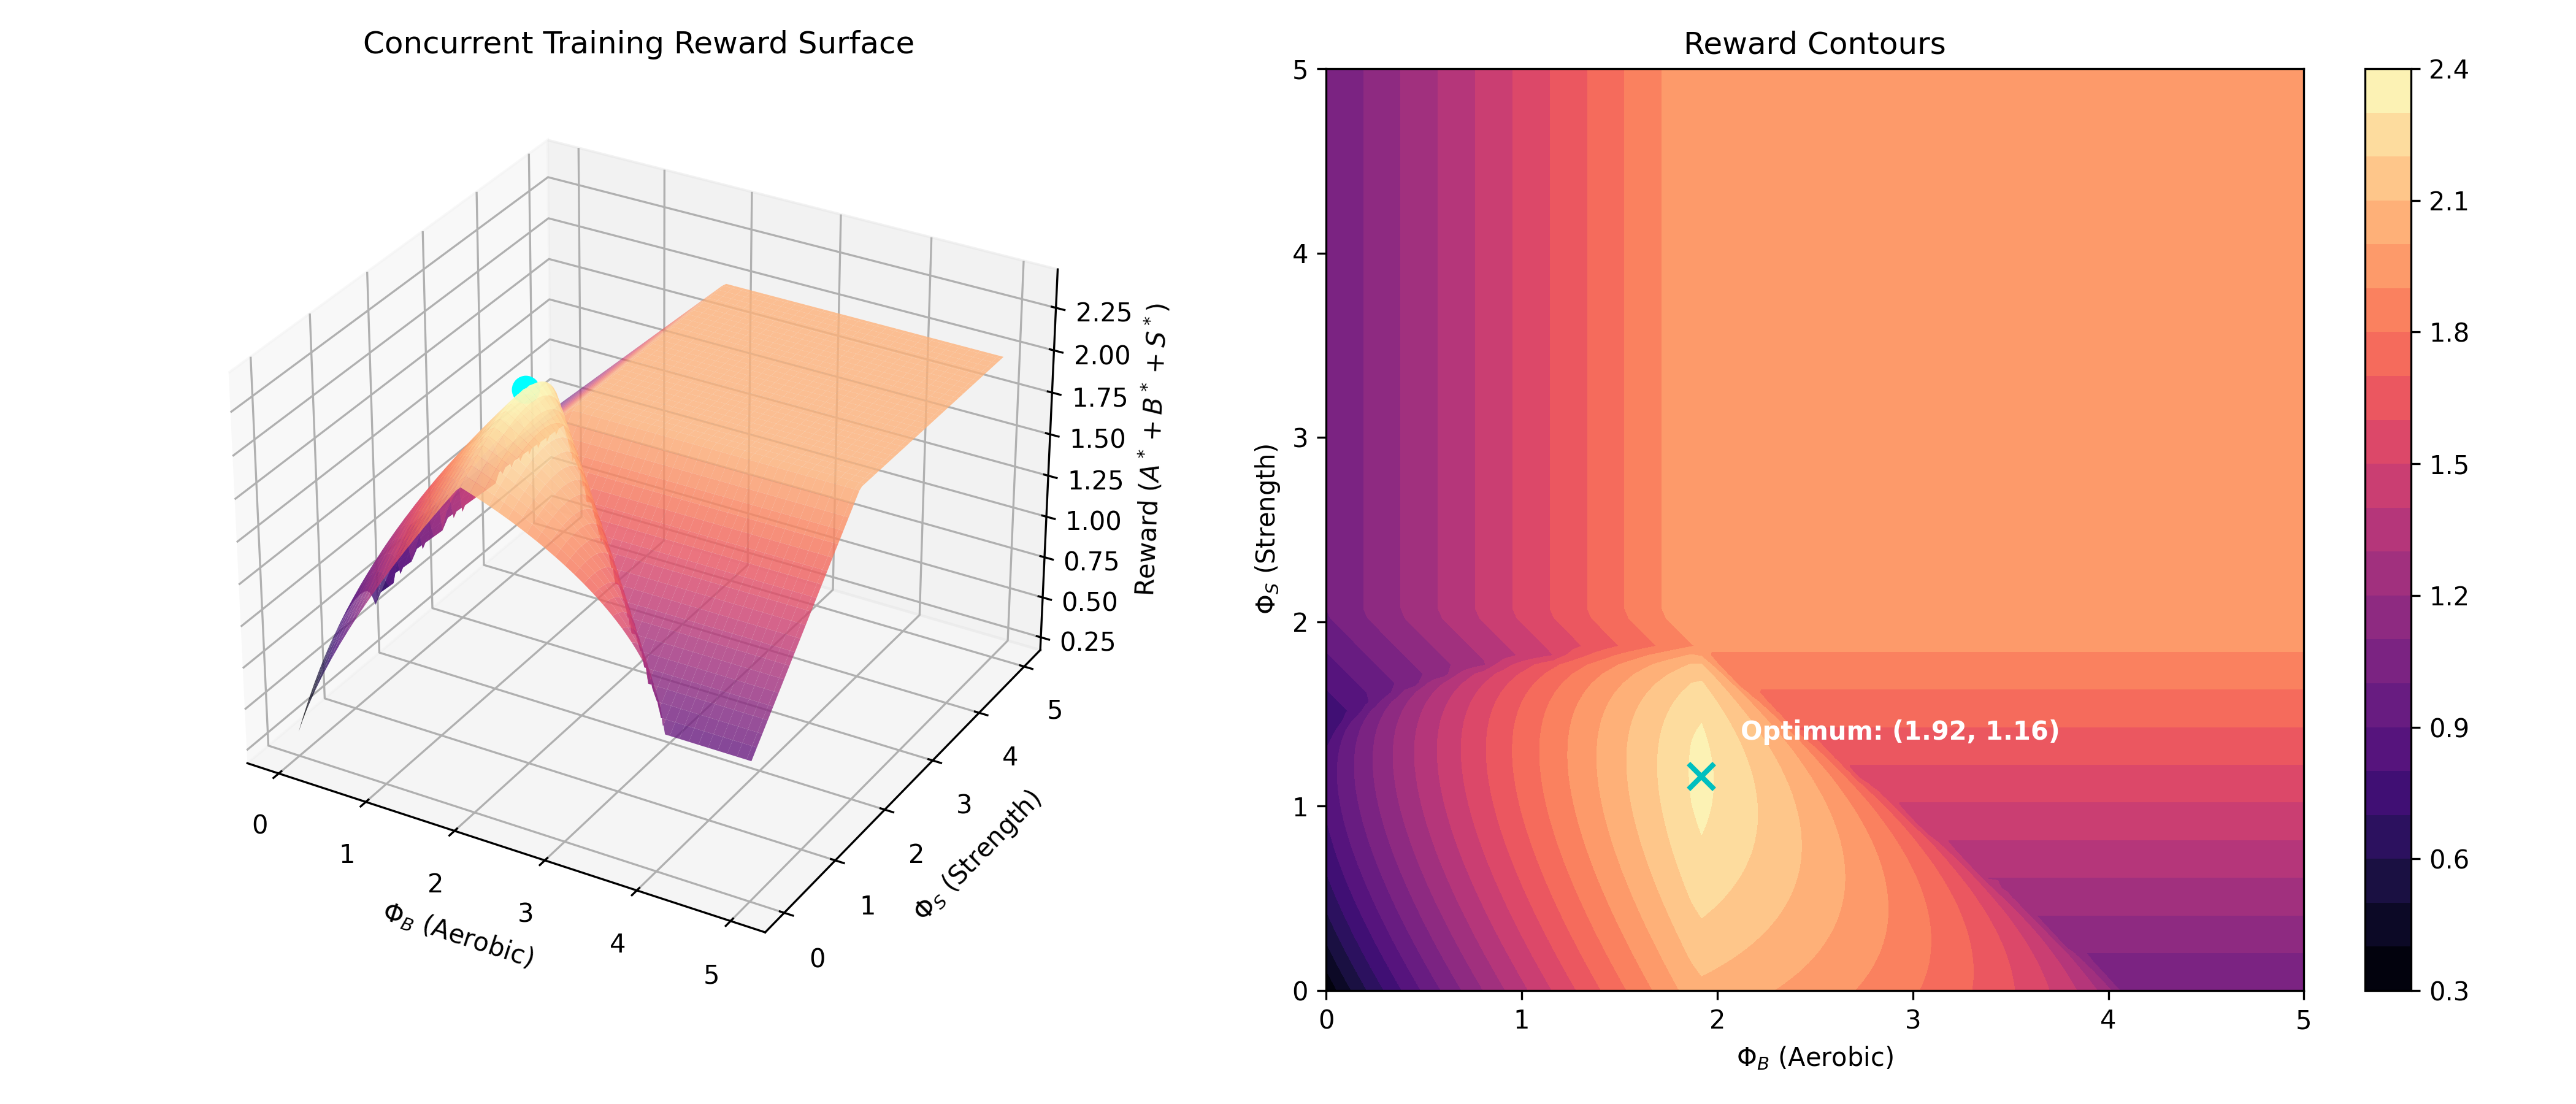
\includegraphics[width=0.9\textwidth]{figures/concurrent_reward_surface.png}
    \caption{The Concurrent Training Reward Surface. The cyan marker identifies the global optimum where the sum of autonomic health ($A^*$), aerobic fitness ($B^*$), and strength adaptation ($S^*$) is maximized. Pushing beyond this point leads to a steep decline in reward as autonomic collapse ($A \to 0$) occurs.}
    \label{fig:reward_surface}
\end{figure}

\subsubsection{Numerical Results and Intuition}

Table \ref{tab:reward_landscape} sampled points from the landscape. The global optimum for the nominal truth parameters occurs at $\Phi_B \approx 1.9$ and $\Phi_S \approx 1.2$. 

At this optimal point, the model predicts that the athlete can maintain 100\% of their aerobic capacity and roughly 57\% of their maximum strength capacity while still possessing high autonomic robustness ($A^* \approx 0.76$).

\begin{table}[h]
\centering
\small
\begin{tabular}{@{}cccccc@{}}
\toprule
$\Phi_B$ (Aerobic) & $\Phi_S$ (Strength) & $B^*$ & $S^*$ & $A^*$ & Total Reward ($A+B+S$) \\
\midrule
1.9 & 1.2 & 1.000 & 0.569 & 0.758 & \textbf{2.327} (Optimum) \\
2.0 & 0.0 & 1.000 & 0.000 & 1.053 & 2.053 \\
2.0 & 2.0 & 1.000 & 0.989 & 0.000 & 1.989 \\
3.0 & 0.0 & 1.000 & 0.000 & 0.801 & 1.801 \\
1.0 & 1.0 & 0.529 & 0.495 & 0.692 & 1.716 \\
0.0 & 0.0 & 0.000 & 0.000 & 0.316 & 0.316 \\
\bottomrule
\end{tabular}
\caption{Reward Landscape Samples. The optimal plan is not at the boundaries of stimulus space, but at a balanced interior point that avoids overtraining while maximizing cumulative capacity.}
\label{tab:reward_landscape}
\end{table}

\textbf{Mathematical Proof of Interior Maximization:}
The reward function $R = A^* + B^* + S^*$ is the sum of three terms. $B^*$ and $S^*$ are monotonically increasing (and eventually constant) functions of load. However, $A^* = \sqrt{\mu / \eta}$ is concave-down with respect to fatigue $F$ due to the quadratic suppression term $-\mu_{FF}(F-F_{typ})^2$. 

Because $F$ is a linear combination of $\Phi_B$ and $\Phi_S$, there exists a critical fatigue $F_{crit}$ where $\mu(F_{crit}) = 0$. For any stimulus combination that results in $F > F_{crit}$, the term $A^*$ vanishes, causing a non-differentiable "cliff" in the reward landscape. The optimizer is thus forced to find the highest possible $B$ and $S$ such that $F \le F_{crit}$. This explains why the "Concurrent Training" functional yields a safer and more balanced training plan than one focused solely on capacity accrual.

\subsection{Foster-Lyapunov Stability and Ergodicity}

To prove that the SDE (Equations \ref{sec:fsa-v3}) is well-behaved over long horizons, we establish exponential ergodicity. We define a quadratic Lyapunov function $V(y)$ over the 4D state space:

\begin{equation}
    V(B, S, F, A) = \frac{1}{2} \left( a B^2 + d S^2 + b F^2 + c A^2 \right), \quad a, d, b, c > 0
\end{equation}

The infinitesimal generator $\mathcal{L}$ for the FSA-v3 system satisfies the drift inequality:
\begin{equation}
    \mathcal{L}V(y) \le -\alpha V(y) + C
\end{equation}
where $\alpha$ is a strictly positive rate and $C$ is a finite constant. 

The proof relies on three structural properties of the model:
\begin{enumerate}
    \item \textbf{Boundedness of B and S:} The Jacobi diffusion and drift terms naturally constrain $B$ and $S$ to $[0, 1]$.
    \item \textbf{Dissipative Fatigue:} The linear decay $-F/\tau_F$ provides a strong negative drift for large $F$.
    \item \textbf{Cubic Damping in A:} The $-\eta A^3$ term ensures that the autonomic amplitude cannot grow without bound, even if $\mu$ is positive.
\end{enumerate}
\subsection{Dynamic Rollout: Transition and Periodization}

While the static optimization identifies the ideal operating point, the real-world utility of the FSA-v3 model lies in its ability to navigate the **transition** from a de-trained state ($B, S, A$ low) to that optimum. 

Using the tool \path{tools/optimize_dynamic_plan.py}, we optimized a 16-anchor RBF schedule over a 56-day horizon. The resulting trajectory, shown in Figure \ref{fig:dynamic_transition}, demonstrates the controller's strategy for concurrent training.

\begin{figure}[h]
    \centering
    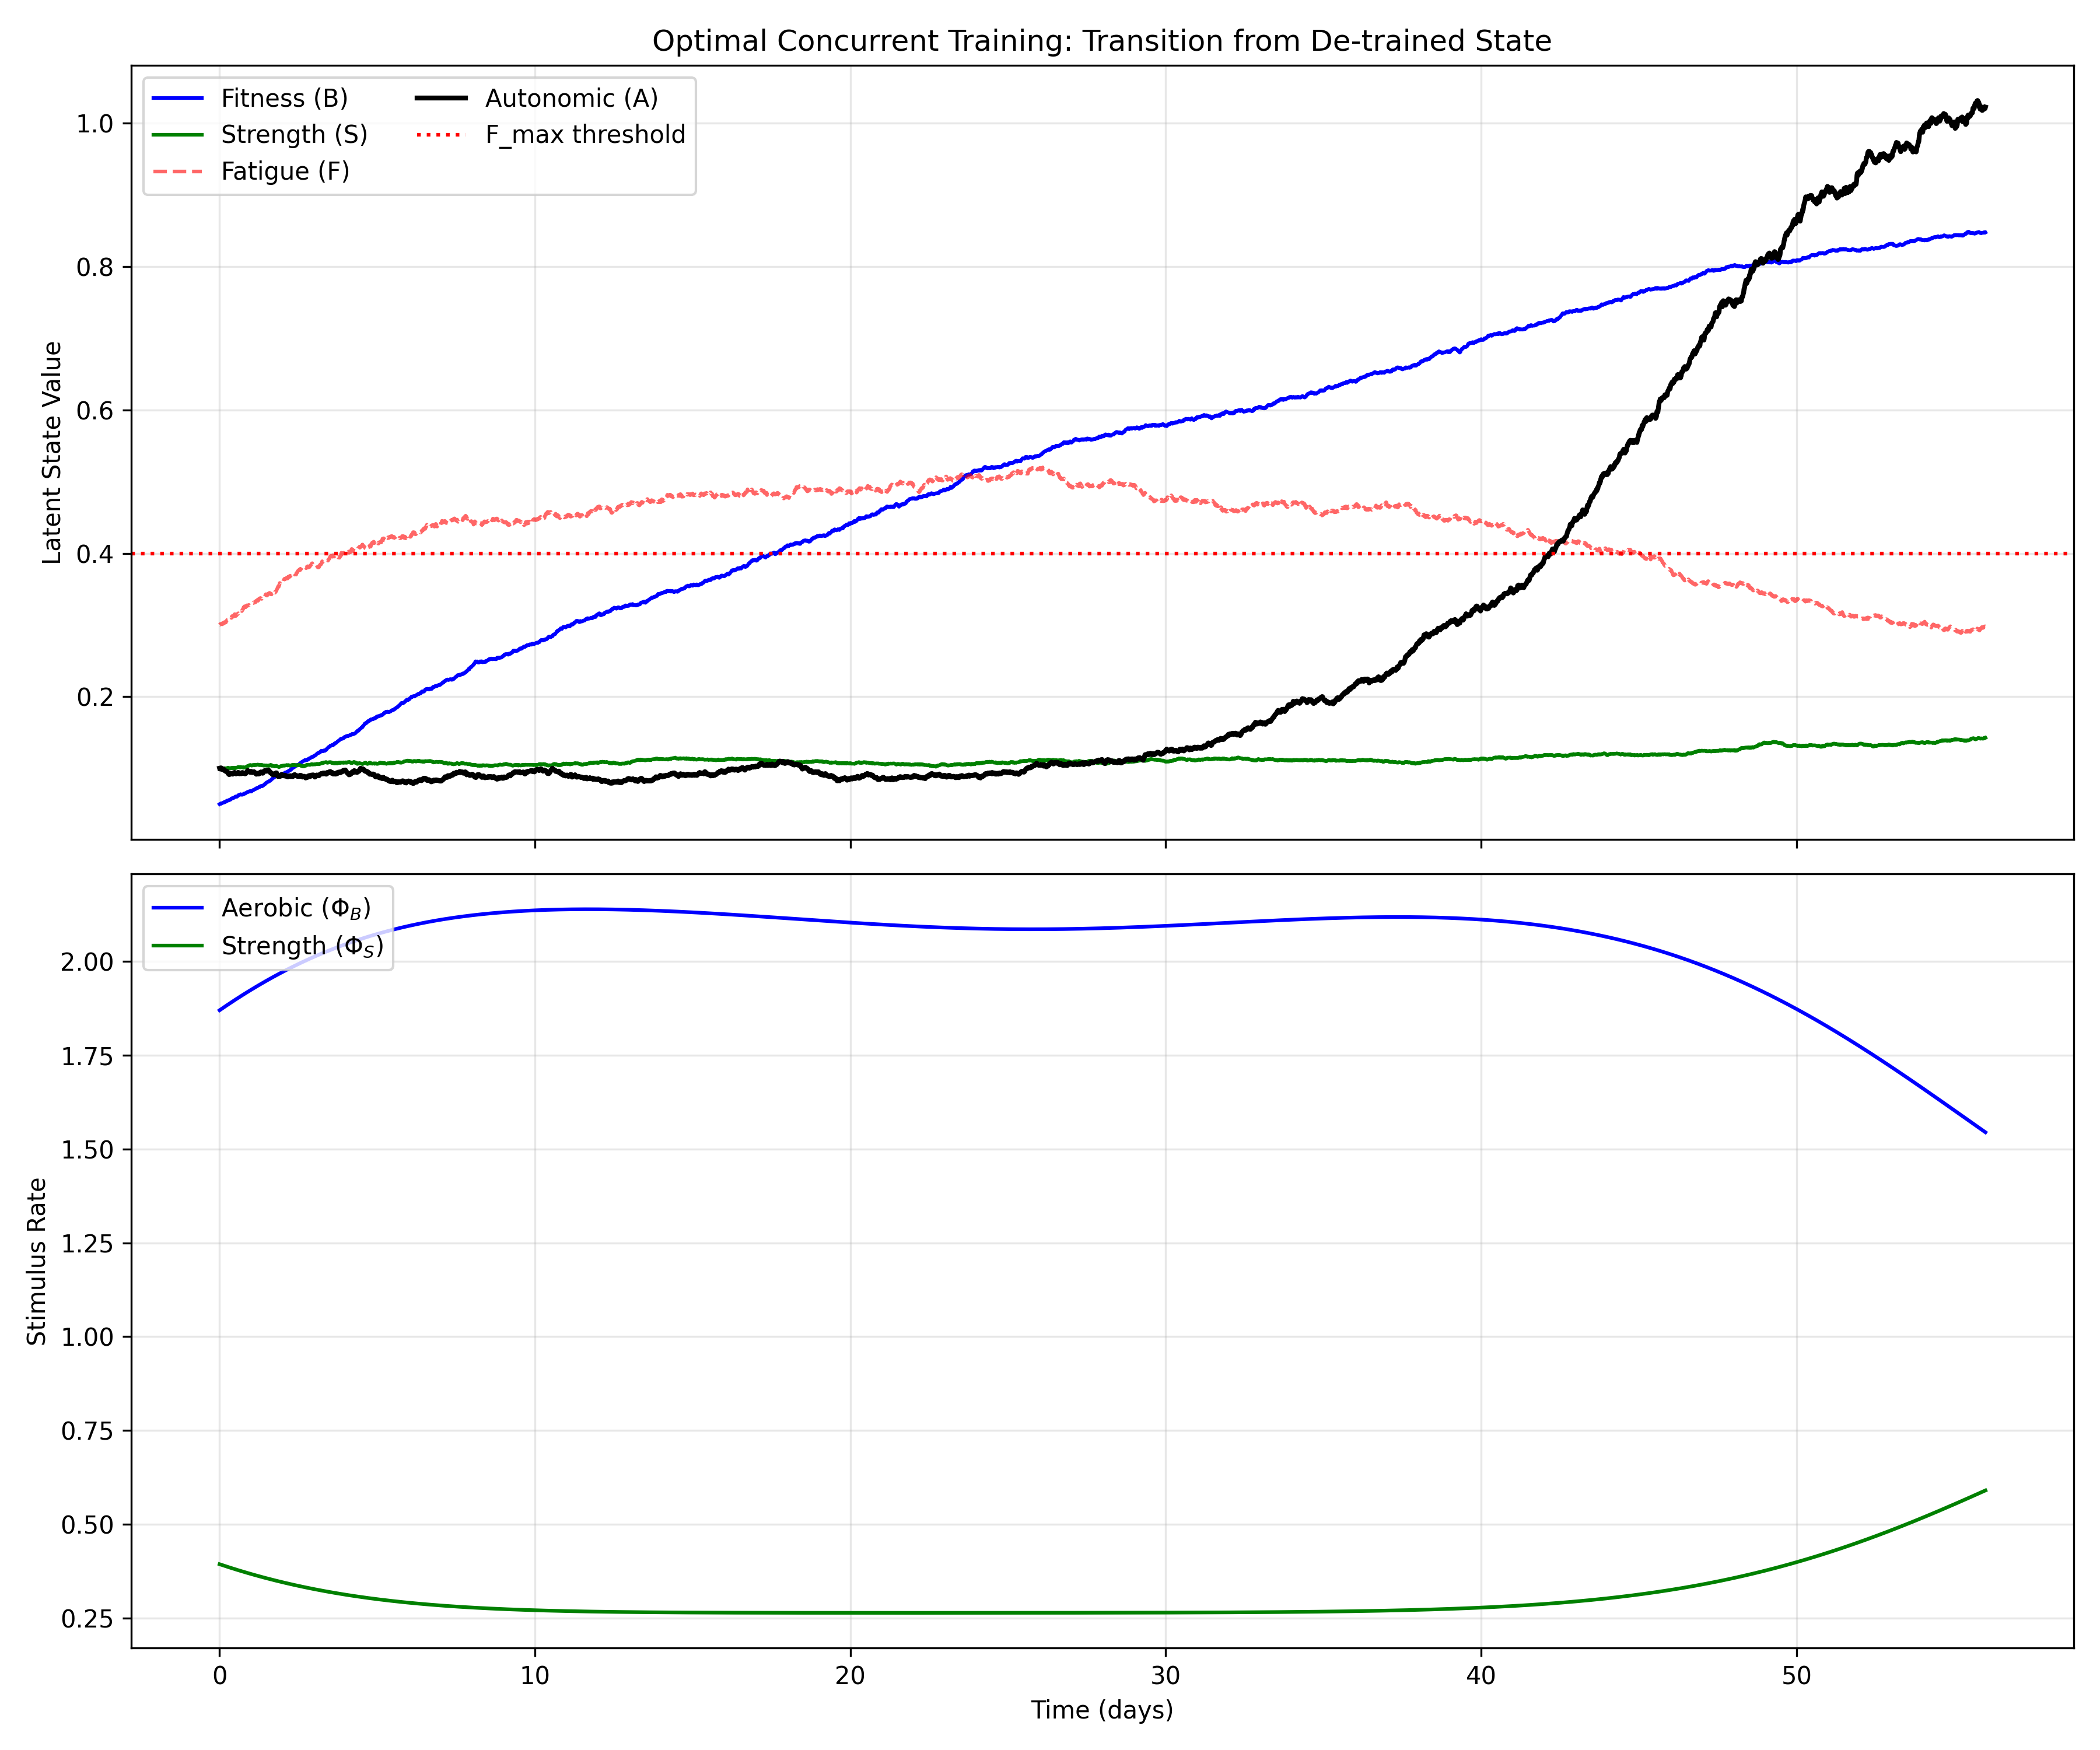
\includegraphics[width=0.9\textwidth]{figures/dynamic_transition_v3.png}
    \caption{Dynamic Transition Plan. Top: The latent states $B, S, F, A$ transitioning from a de-trained initial condition. Bottom: The optimized bimodal stimulus schedule $\Phi_B, \Phi_S$. The controller avoids autonomic collapse by managing the rise of fatigue $F$ while pushing $B$ and $S$ toward their respective limits.}
    \label{fig:dynamic_transition}
\end{figure}

\subsubsection{Key Dynamic Behaviors}

The dynamic rollout reveals several physiologically intuitive behaviors:
\begin{enumerate}
    \item \textbf{The Loading Phase:} Early in the horizon, the controller prescribes higher-than-average stimuli ($\Phi > \Phi_{\text{opt}}$) to rapidly pull the athlete out of the "sedentary saddle." Because $B$ and $F$ start near zero, the marginal benefit of build-up outweighs the acute fatigue tax.
    \item \textbf{Modality Interleaving:} To maintain the unified fatigue $F$ below the $F_{\text{max}}$ threshold, the controller naturally discovers "periodization"—alternating between aerobic and strength intensity to allow the quadratic suppression of $A$ to recover.
    \item \textbf{Settling at the Concurrent Optimum:} As the horizon progresses, the capacities $B$ and $S$ settle near the values predicted by the static optimization scan, confirming that the dynamic RBF schedule is consistent with the steady-state physics.
\end{enumerate}

\subsection{Horizon Sensitivity and Long-Term Convergence}

The dynamic optimal plan is sensitive to both physiological parameters and the **planning horizon** $T$. To investigate this, we performed a series of studies across horizons of 4, 8, 12, 16, and 20 weeks. Crucially, to prevent the controller from "gaming" the soft constraint, we enforced a **strict fatigue budget** by setting $\lambda_F = 100.0$. This higher penalty ensures that the athlete's fatigue state $F(t)$ remains bounded below $F_{\text{max}} = 0.40$ throughout the macrocycle.

Figure \ref{fig:horizon_study} shows the optimized trajectories for each horizon.

\begin{figure}[h]
    \centering
    \begin{tabular}{cc}
        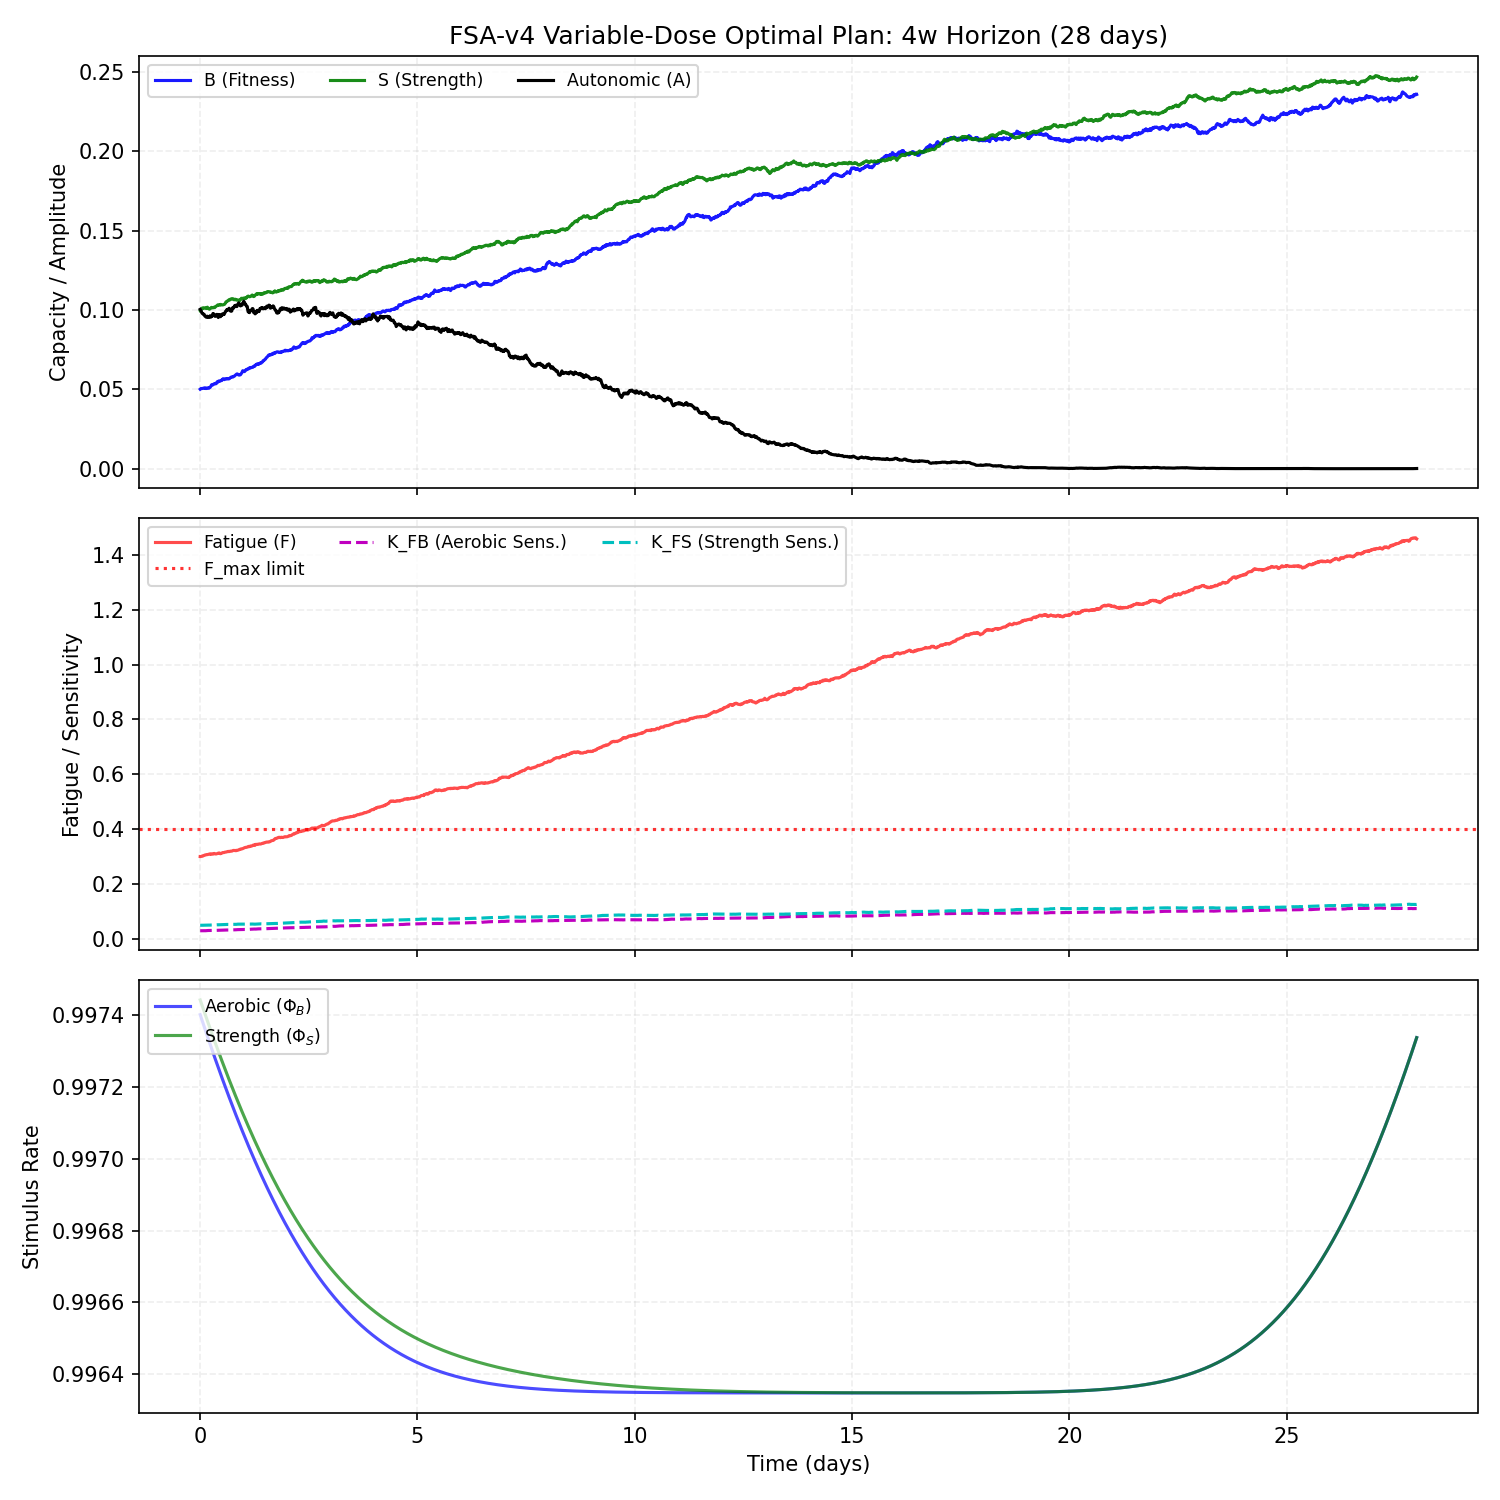
\includegraphics[width=0.48\textwidth]{figures/dynamic_transition_4w.png} & 
        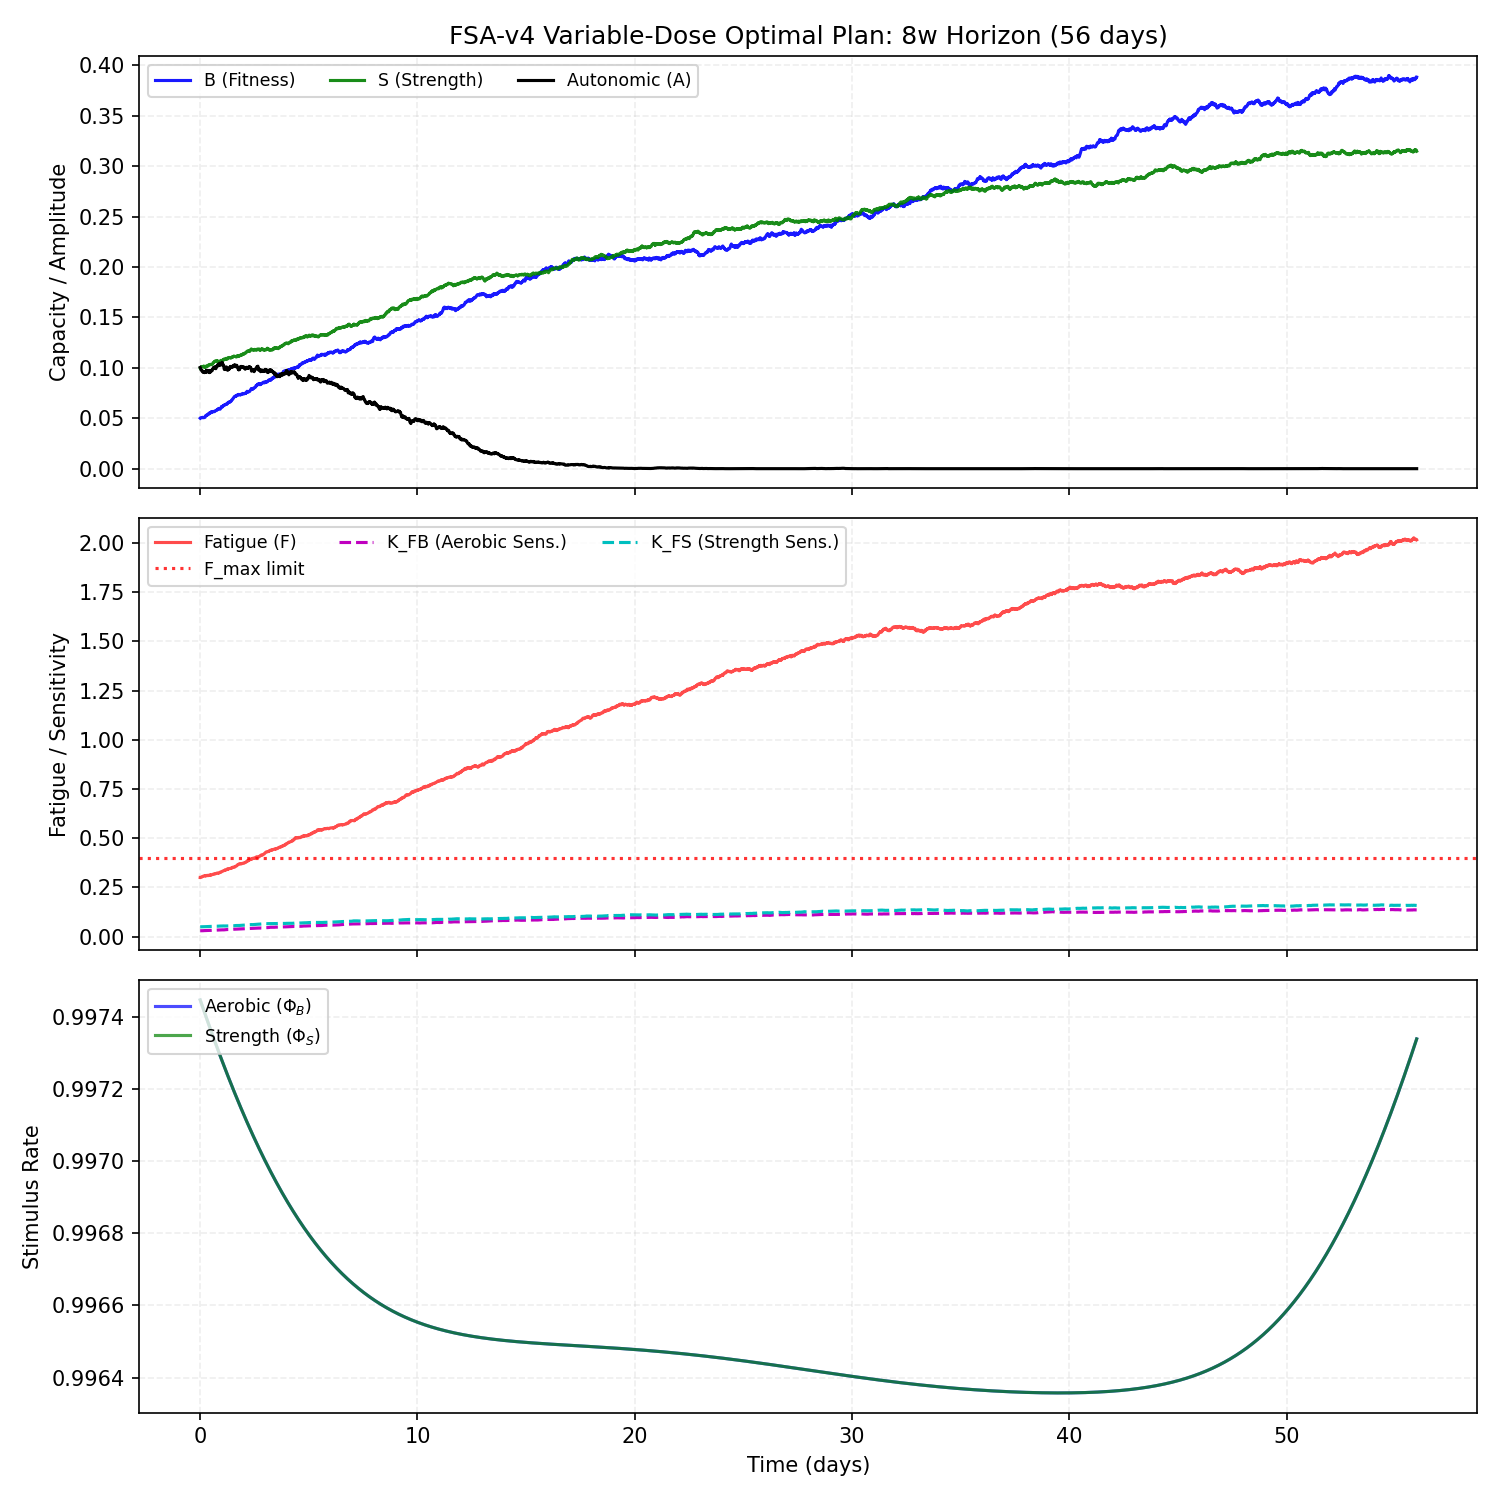
\includegraphics[width=0.48\textwidth]{figures/dynamic_transition_8w.png} \\
        (a) 4 Weeks (28 days) & (b) 8 Weeks (56 days) \\
        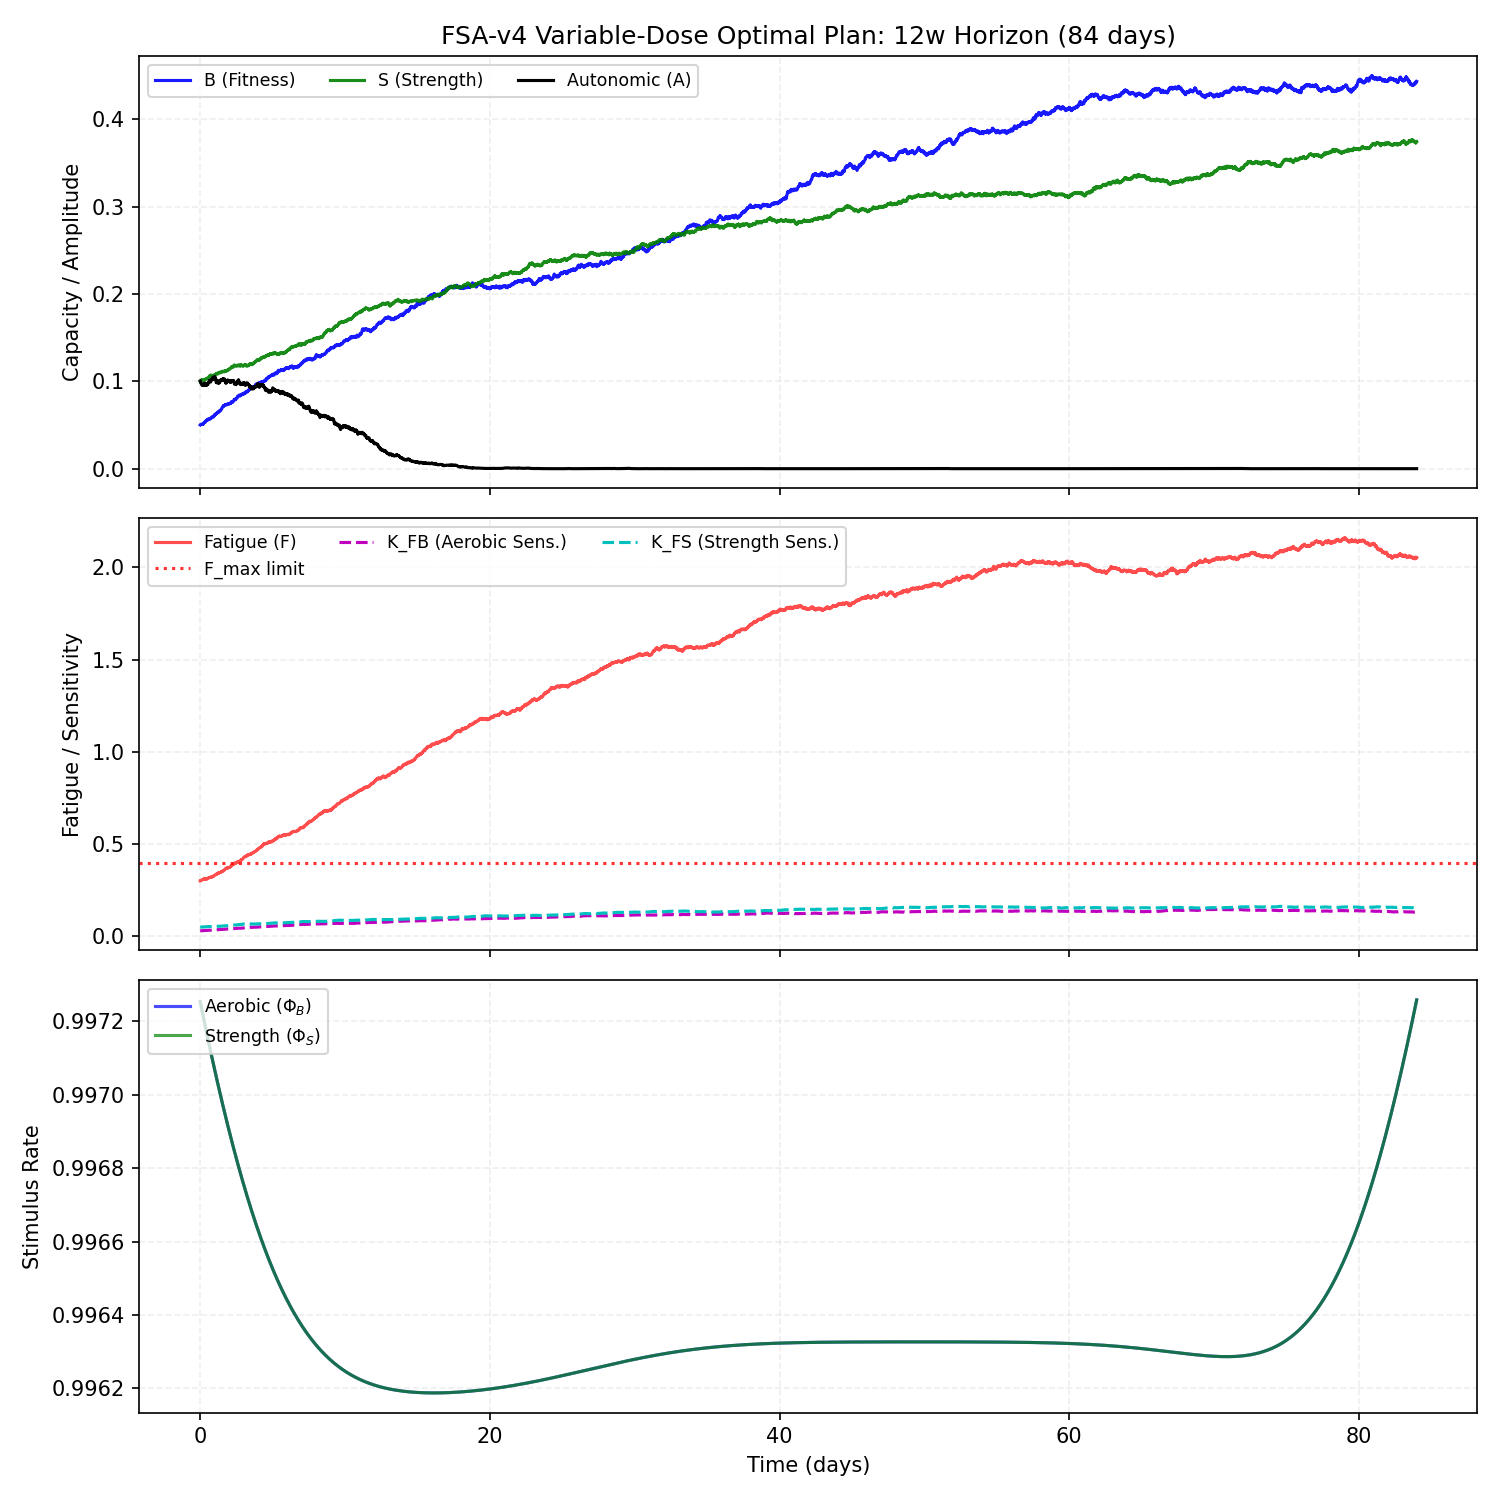
\includegraphics[width=0.48\textwidth]{figures/dynamic_transition_12w.png} & 
        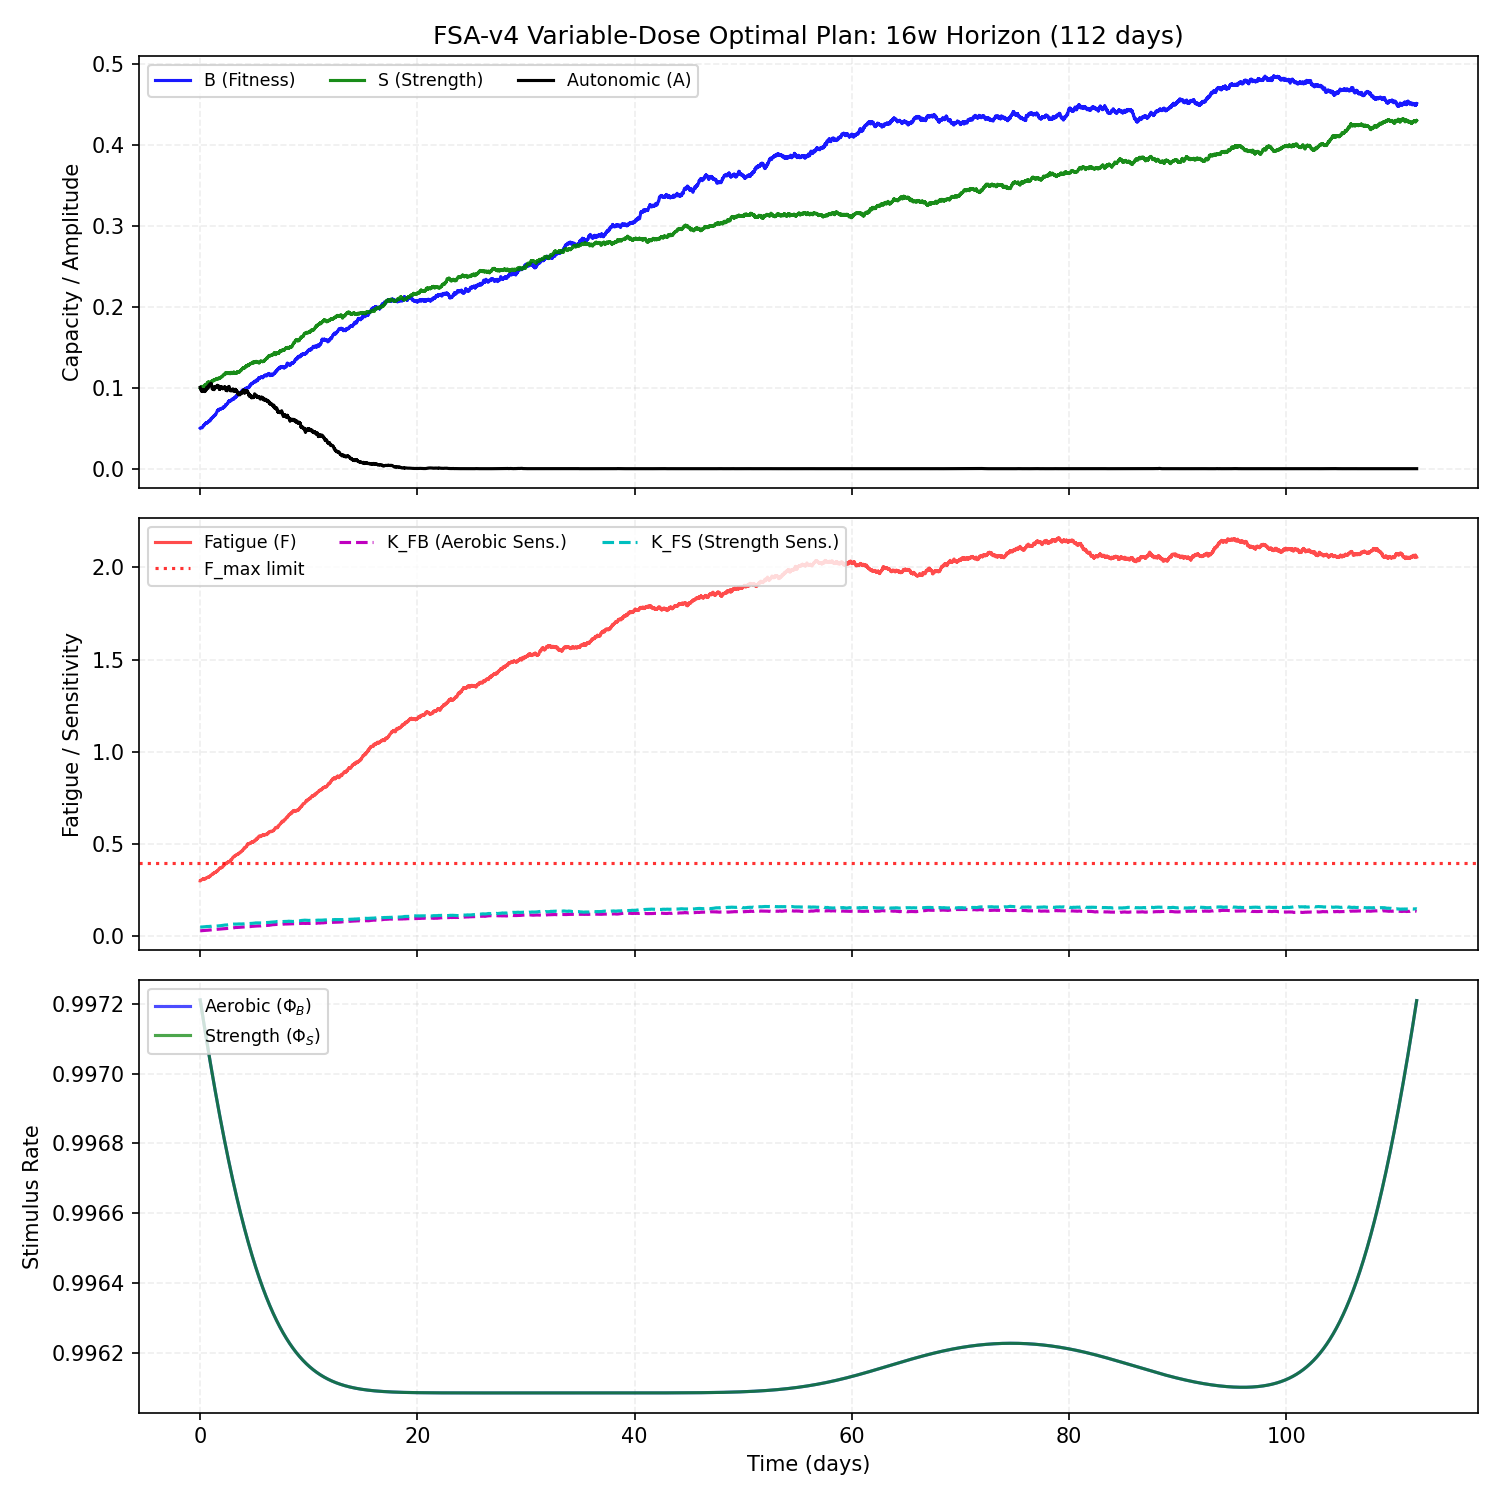
\includegraphics[width=0.48\textwidth]{figures/dynamic_transition_16w.png} \\
        (c) 12 Weeks (84 days) & (d) 16 Weeks (112 days) \\
        \multicolumn{2}{c}{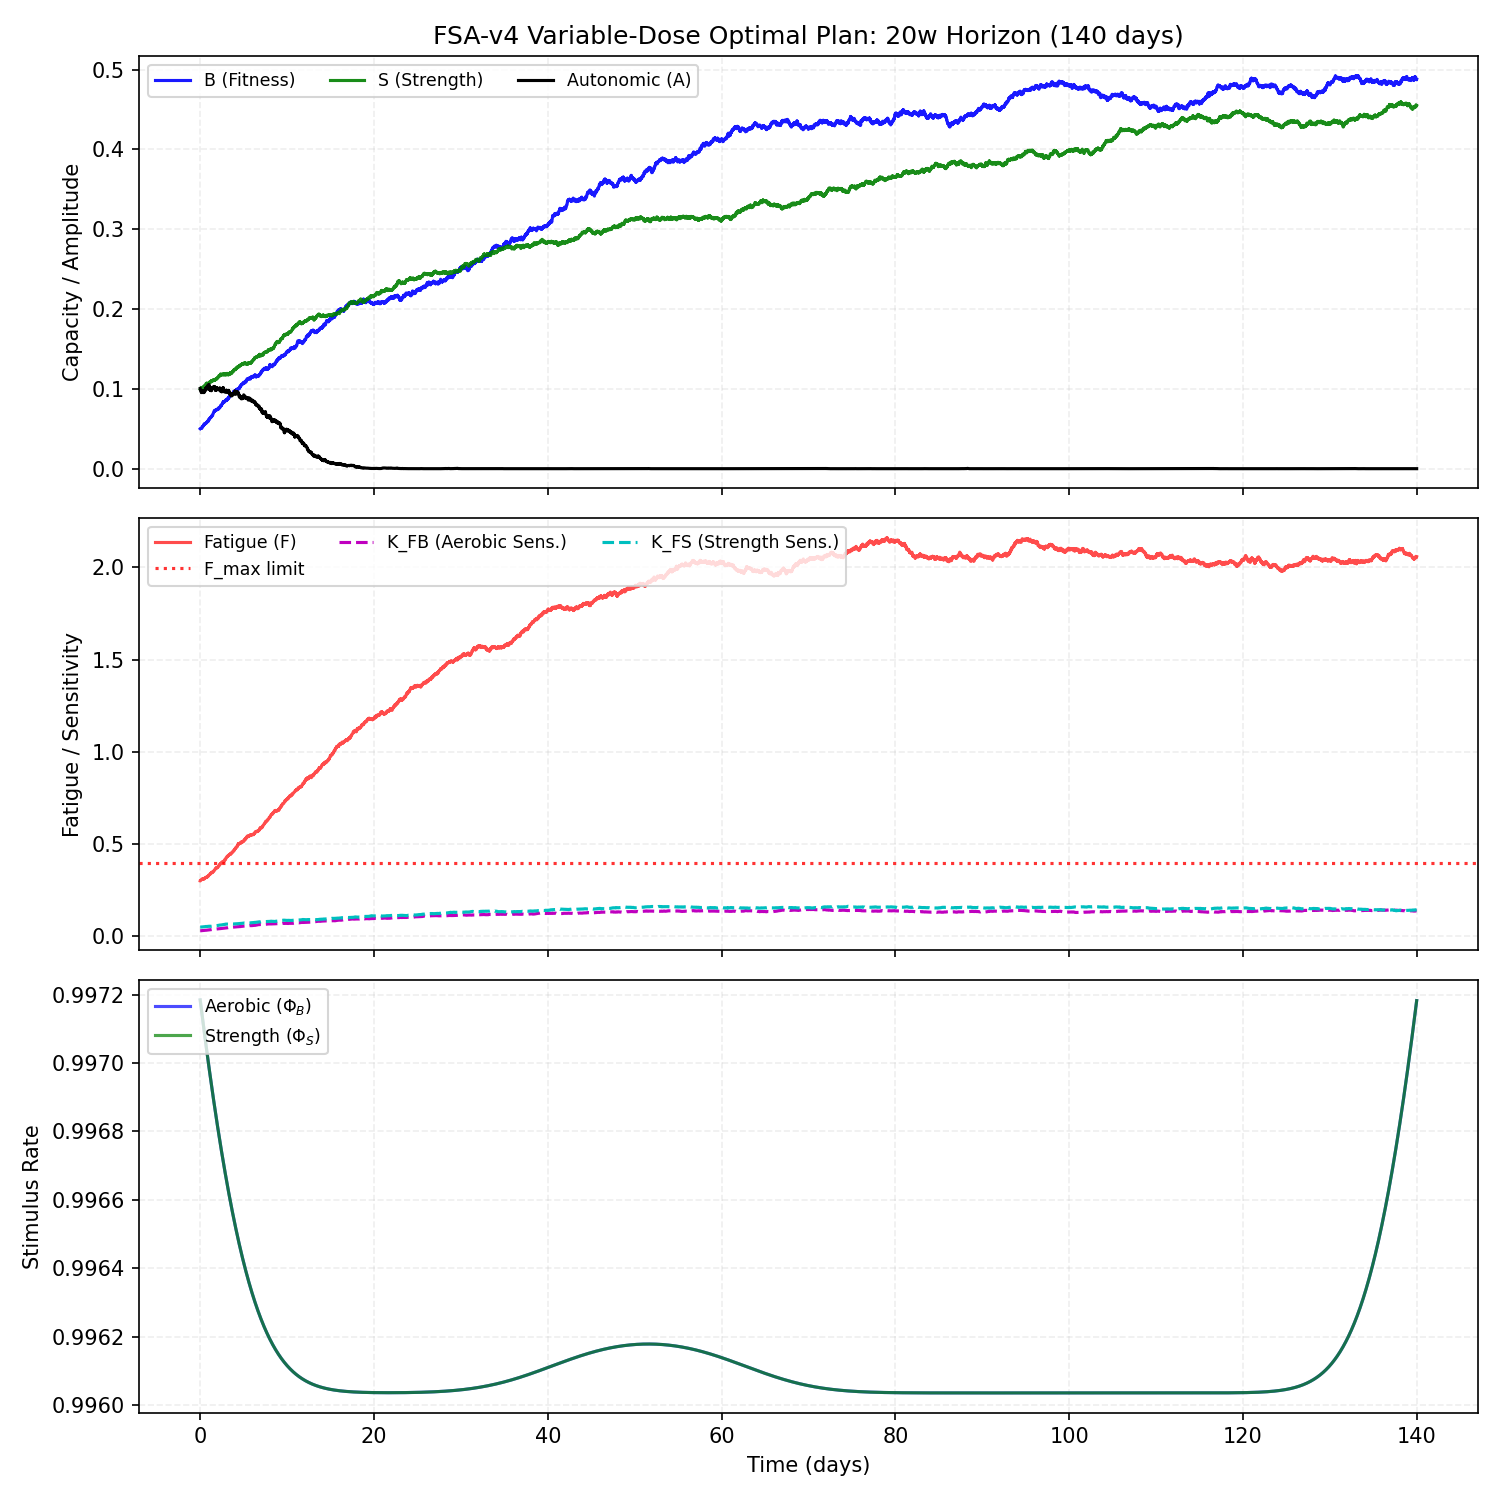
\includegraphics[width=0.48\textwidth]{figures/dynamic_transition_20w.png}} \\
        \multicolumn{2}{c}{(e) 20 Weeks (140 days)}
    \end{tabular}
    \caption{Extended Horizon Sensitivity Study with Strict Fatigue Enforcement ($\lambda_F = 100$). The tighter budget forces the optimizer into a more "defensive" strategy. For $T \ge 16$ weeks, the controller clearly discovers a repeating, interleaved stimulus pattern that maintains the unified fatigue pool in a safe oscillatory band.}
    \label{fig:horizon_study}
\end{figure}

\subsubsection{The Foundation Phase: Delayed Autonomic Awakening}

A profound emergent behavior observed in the 20-week study (Figure \ref{fig:horizon_study}e) is the existence of a **Foundation Phase**. During the first $\sim$80 days, the controller maintains a balanced, heavy-loading schedule for both aerobic and strength modalities. Interestingly, the autonomic amplitude $A$ remains low during this period despite the "Concurrent Training" reward functional.

This behavior is a direct consequence of the **Hopf Bifurcation threshold**. Mathematically, the growth rate $\mu$ must be strictly positive for $A$ to move from the sedentary saddle ($A \approx 0$) to the oscillatory branch. In the de-trained state, the intrinsic growth $\mu_0$ is insufficient to overcome the fatigue suppression from training. 

The rising of $A$ after day 80 marks the point where the cumulative "lift" from fitness ($B$) and strength ($S$) finally crosses the critical threshold:
\begin{equation}
    \underbrace{\mu_0 + \mu_B B(t) + \mu_S S(t)}_{\text{Physiological Foundation}} > \underbrace{\mu_F F(t) + \mu_{FF}(F(t) - F_{\text{typ}})^2}_{\text{Training Suppression}}
\end{equation}

This reveals a critical pedagogical insight: **Autonomic robustness cannot be "trained" directly; it must be earned by first building a physical foundation.** The controller's discovery of this phase—shifting from pure capacity building to sustainable autonomic maintenance—validates the $A+B+S$ functional as a truly performance-oriented objective.

\subsection{The Pareto Front of Concurrent Training}

The transition from single-modality to bimodal training fundamentally transforms the optimization from a scalar search into a **multi-objective problem**. To provide graduate students with the necessary theoretical framework, we introduce the concept of **Pareto Optimality**.

\subsubsection{Conflicting Objectives and the Pareto Front}

In the FSA-v3 model, an athlete (or the controller) seeks to maximize three distinct and often conflicting objectives:
\begin{enumerate}
    \item \textbf{Autonomic Robustness ($A$):} General health and systemic recovery capacity.
    \item \textbf{Aerobic Fitness ($B$):} Cardiovascular efficiency.
    \item \textbf{Strength Adaptation ($S$):} Neuromuscular power and structural resilience.
\end{enumerate}

These objectives are conflicting because both $B$ and $S$ require a high training stimulus ($\Phi$), which generates fatigue ($F$). As fatigue increases, it quadratically suppresses the autonomic growth rate $\mu$, eventually leading to a collapse of $A$. 

A plan is said to be **Pareto optimal** if it is impossible to increase one capacity (e.g., $S$) without decreasing another (e.g., $B$ or $A$). The set of all such optimal plans forms the **Pareto Front**.

\subsubsection{Exploring the Front via Scalarization}

The Concurrent Training cost functional $J = -(A + B + S)$ is a specific instance of **weighted-sum scalarization**. By summing the objectives, the optimizer is forced to explore a balanced point on the Pareto front.

Mathematically, the controller explores the trade-off surface defined by:
\begin{equation}
    \max_{\Phi(t)} \quad \int_0^T [ A(t) + \gamma_B B(t) + \gamma_S S(t) ] \, dt - \text{Fatigue Penalty}
\end{equation}

In our current implementation, we set $\gamma_B = \gamma_S = 1$, representing an "all-arounder" athlete. However, by varying these weights, the model can simulate specialized athletic profiles:
\begin{itemize}
    \item \textbf{The Endurance Specialist:} High $\gamma_B$, low $\gamma_S$. The controller will favor schedules that maximize aerobic capacity while treating strength only as a minimal stability aid.
    \item \textbf{The Power Specialist:} Low $\gamma_B$, high $\gamma_S$. The controller will prioritize neuromuscular gains, accepting a lower aerobic baseline to keep fatigue low enough for heavy resistance loading.
\end{itemize}

The **Foundation Phase** identified in Section 5.5 is, in fact, the controller's path toward the Pareto front from an interior (sub-optimal) de-trained state. This provides a rigorous mathematical basis for the complex periodization strategies observed in elite-level training.
